%!TEX root = ../thesis.tex
\section{SOFTWARE REQUIREMENTS SPECIFICATION}

The software development process starts with writing a software requirements specification (SRS) so
that it serve as an agreement between client and contractor about the set of the features which need
to be implemented. Another important purpose of this document is to create understanding of the
features with higher and lower priority, thus developer would know what should be implemented in the
first version of the product and what could be added later.

In this section the simplified version of the SRS will be presented which includes description
of the user interface, operating environment, and set of system features with detailed
explanation.

\subsection{Graphical User Interface}

The interface design was provided by Mathrioshka LLC, which includes set of different states
of the application with small description provided. The interface should be implemented
to work in a browser with use of HTML~5 standard. The whole program should be implemented
as single page application, which means that all changes in the state of the application
happen without page reload. The interface have to be responsive and support screen sizes
starting from $800 \times 600$ pixels.

The manipulation of the data within the application is performed utilizing main control elements.
Most important elements are listed below:

\begin{enumerate}
  \item Mode selector is needed for switching from general overview to location-wise analysis and
  placed in the left bottom corner of the screen.

  \begin{figure}[ht]
    \centering
    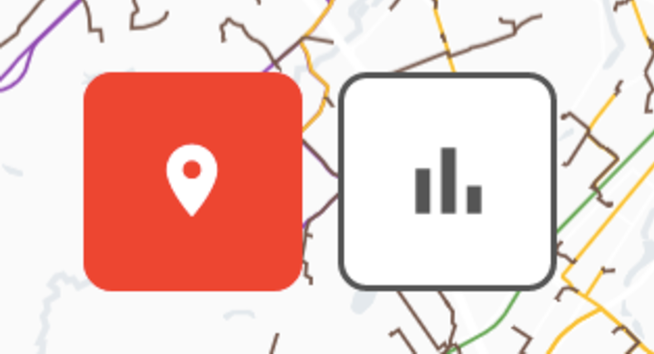
\includegraphics[width=0.33\textwidth]{mode-selector.pdf}
    \caption{Mode selector.}
    \label{pic:mode_selector}
  \end{figure}

  \item Overview mode selector switches different types of overview analysis tools. For some
  views it has embedded slider used for filtering. The component is positioned on the right
  side of the screen.

  \begin{figure}[ht]
    \centering
    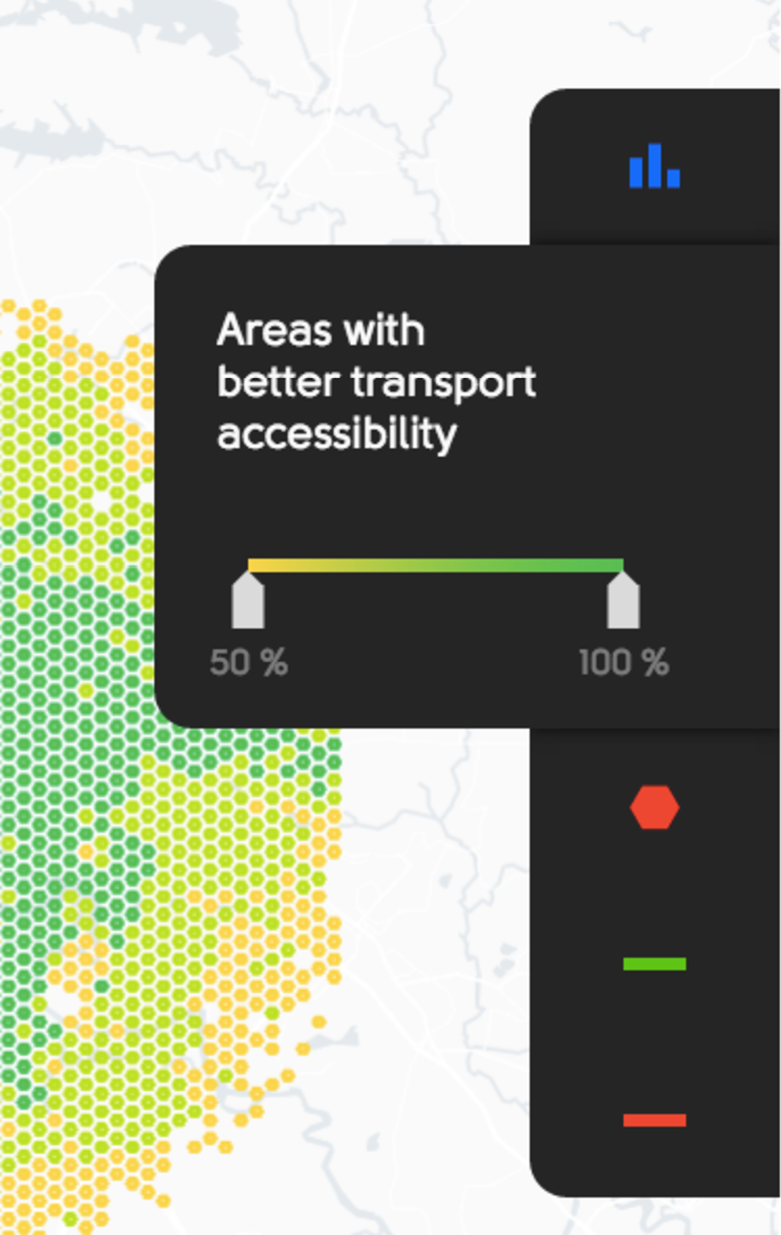
\includegraphics[width=0.25\textwidth]{overview-mode.pdf}
    \caption{Overview mode selector.}
    \label{pic:overview_selector}
  \end{figure}

  \item Transport filter is a set of checkboxes where every checkbox represents a certain
  type of transport. This component is placed on top of the screen.

  \begin{figure}[ht]
    \centering
    
\includegraphics[width=0.8\textwidth]{transport-filter.pdf}
    \caption{Transport filter.}
    \label{pic:transport_filter}
  \end{figure}

  \item Current location indicator shows what point is selected on the map at this moment and
  also allows to clear current selection. The component is located on the right side of the window.

  \begin{figure}[ht]
    \centering
    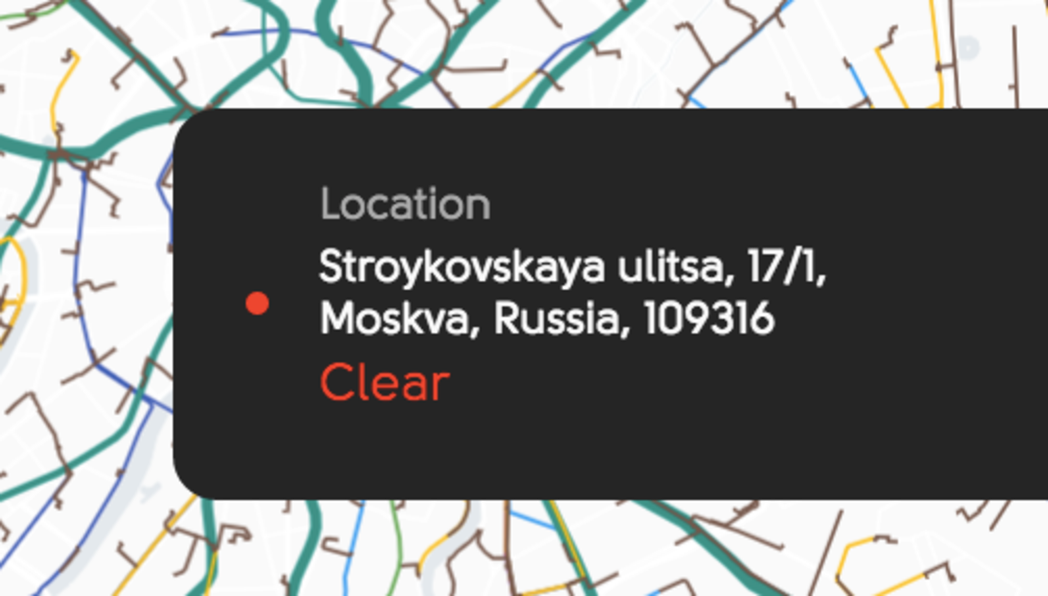
\includegraphics[width=0.3\textwidth]{location-selector.pdf}
    \caption{Current location indicator.}
    \label{pic:location_selector}
  \end{figure}

  \item Map is the most important element of the interface which is presented on every screen
  of the application and the only thing that changes is the content of the map.
  This component can show points, areas, routes and also provides functionality for
  selecting particular locations for analysis.

  \begin{figure}[ht]
    \centering
    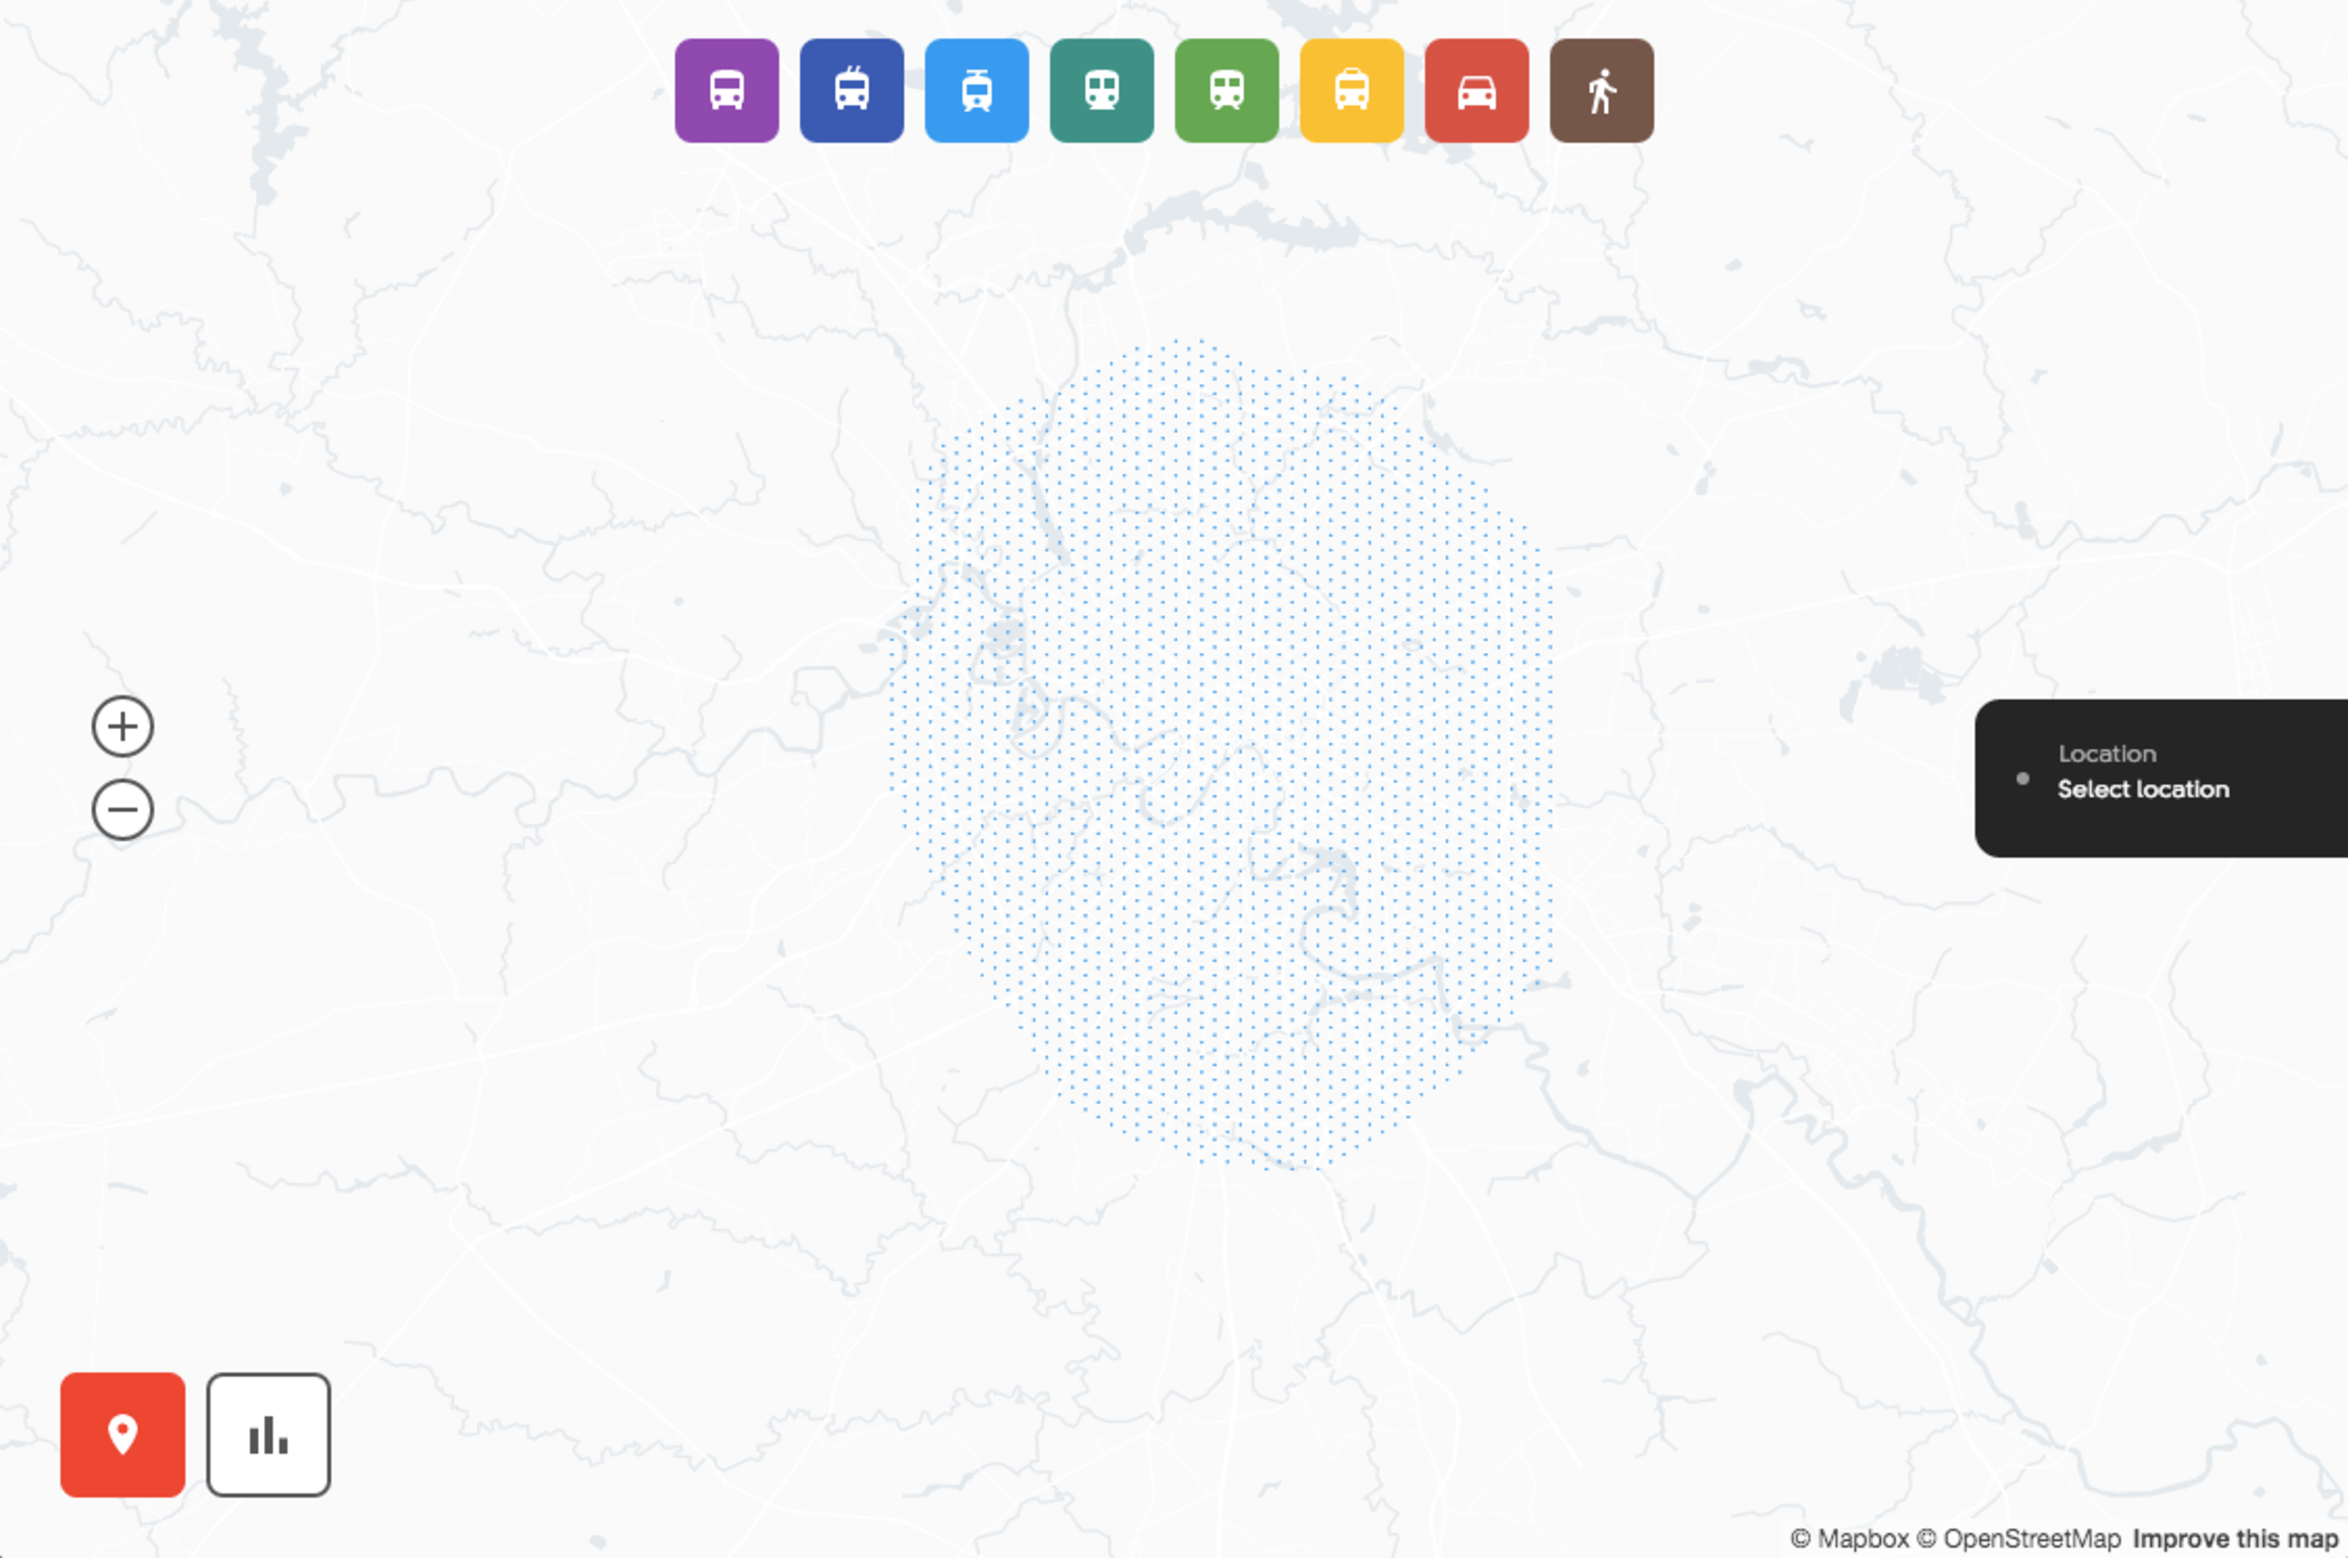
\includegraphics[width=0.80\textwidth]{map.pdf}
    \caption{Map.}
    \label{pic:map}
  \end{figure}

\end{enumerate}

\subsection{Operating Environment}

The software is developed on x86 based computer using Mac OS X 10.11 operating system. The
computer hardware is featured 8~GB 1600~MHz DDR3 RAM and 1.6 GHz Intel Core i5 processor.
The client should operate on any system which is able to install browsers like Google Chrome~49.0,
Safari, Firefox or Microsoft Edge. Hence it works well on Windows, Mac OS X and Linux. As for the
server, it was tested to work on Ubuntu~14.04 and 512~MB~RAM. Running the server side on Windows
was not tested.

\subsection{System Features}

\begin{description}
  % Feature 1
  \item[Use case 1:] Show all directions from specific location to all other points.

  \underline{\smash{Primary actor:}} User

  \underline{\smash{Main scenario:}}
  \begin{enumerate}
    \item The user enters ``Location analysis'' mode.
    \item The user selects specific point on the grid.
    \item The system displays all routes coming from the selected point to all other points on the
    grid. The routes are colored by the type of transport. The line which represents part
    of the route has a width depending on weight of the current line. The weight is calculated
    as occurrence of this line in all possible routes. More precisely, if two different
    routes are going over particular line it means that the weight of this line will
    be equal to two. In other words the wider the line, the more this line is used in all other
    directions (routes) calculated for all points on the grid to all other points.
    \item The user is able to filter lines by transport type.
    \item The user is able to switch color mode from coloring by transport to
    coloring by speed.
  \end{enumerate}

  % Feature 2
  \item[Use case 2:] Show prevailing transport

  \underline{\smash{Primary actor:}} User

  \underline{\smash{Main scenario:}}
  \begin{enumerate}
    \item The user enters ``General overview'' mode.
    \item The user selects ``Prevailing transport'' option.
    \item The grid of markers is displayed. Each marker is associated with one
    point on the grid. The markers are colored accordingly to certain transport type. Prevailing
    transport is defined by calculating total time spent in particular transport when
    moving from current points to all other points on the grid.
    \item The user is able to filter markers by transport type.
  \end{enumerate}

  % Feature 3
  \item[Use case 3:] Most accessible locations

  \underline{\smash{Primary actor:}} User

  \underline{\smash{Main scenario:}}
  \begin{enumerate}
    \item The user enters ``General overview'' mode.
    \item The user selects ``Most accessible locations'' option.
    \item The grid of markers is displayed. Each marker is associated with one
    point on the grid. The markers are colored accordingly to accessibility level of the
    certain point. Accessibility is defined as total time spent in transport when user
    moves from current points to all other points on the grid. Once accessibility
    is calculated for all points the value is scaled to 0 to 100\%.
    \item The user is able to filter markers by accessibility level from 50\% to 100\%.
  \end{enumerate}

  % Feature 4
  \item[Use case 4:] Least accessible locations

  \underline{\smash{Primary actor:}} User

  \underline{\smash{Main scenario:}}
  \begin{enumerate}
    \item The user enters ``General overview'' mode.
    \item The user selects ``Least accessible locations'' option.
    \item The grid of markers is displayed. Each marker is associated with one
    point on the grid. The markers are colored accordingly to accessibility level of the
    certain point. Accessibility is defined as total time spent in transport when user
    moves from current points to all other points on the grid. Once accessibility
    is calculated for all points the value is scaled to 0 to 100\%.
    \item The user is able to filter markers by accessibility level from 0\% to 50\%.
  \end{enumerate}

  \underline{\smash{Comments:}} This feature is very similar to 3rd use case except
  the color scheme is different and filtering is preformed within other percentage range.

  % Feature 5
  \item[Use case 5:] Fastest parts of the routes

  \underline{\smash{Primary actor:}} User

  \underline{\smash{Main scenario:}}
  \begin{enumerate}
    \item The user enters ``General overview'' mode.
    \item The user selects ``Fastest parts of the routes'' option.
    \item All of the lines (routes) are displayed which has speed in a range from
    20 km/h to 40 km/h. The lines are colored differently from yellow to green
    depending on the speed.
    \item The user is able to filter lines by speed using slider control.
  \end{enumerate}

  % Feature 6
  \item[Use case 6:] Slowest parts of the routes

  \underline{\smash{Primary actor:}} User

  \underline{\smash{Main scenario:}}
  \begin{enumerate}
    \item The user enters ``General overview'' mode.
    \item The user selects ``Slowest parts of the routes'' option.
    \item All of the lines (routes) are displayed if the speed is in the range from
    0 km/h to 20 km/h. The lines are colored differently from dark red to light red
    depending on the speed.
    \item The user is able to filter lines by speed using slider control.
  \end{enumerate}
\end{description}